\documentclass[12pt]{llncs}

\usepackage{makeidx}  % allows for indexgeneration
\usepackage{geometry}
\geometry{a4paper, top=20mm, left=20mm, right=20mm, bottom=20mm,
headsep=10mm, footskip=12mm}
\makeatletter 
\renewcommand\section{\@startsection 
   {section}{1}{0mm}%         % name, ebene, einzug 
   {1\baselineskip}%            % vor-abstand 
   {0.5\baselineskip}%            % nach-abstand 
   {\bfseries\Large}%      % layout 
   } 
\makeatother 
\makeatletter 
\renewcommand\subsection{\@startsection 
   {subsection}{2}{0mm}%      % name, ebene, einzug 
   {0.7\baselineskip}%            % vor-abstand 
   {0.5\baselineskip}%            % nach-abstand 
   {\bfseries\large}%           % layout 
   } 
\makeatother 

%\bibliographystyle{splncs}
\usepackage{graphicx}
\title{Accessible EPUB : Making EPUB 3 documents universal accessible}
\author{Thorsten Schwarz \and Sachin Rajgopal \and Rainer Stiefelhagen}

\institute{Karlsruhe Institute of Technology, Studycentre for the Visually Impaired, Engesserstr. 4, 76131 Karlsruhe, Germany\\
\email{thorsten.schwarz@kit.edu},\\ WWW home page:
\texttt{http://szs.kit.edu}
}

\begin{document}

\maketitle

\begin{abstract}
Current document standards have the characteristic that they can only serve one group of users under the aspect of vision (sighted, visually impaired or blind reader). Wouldn't it be nice if one documentformat could combine all properties in one document? 
This paper presents a new approach of an universal accessible version of EPUB 3 documents, which will allow sighted, visually impaired and blind readers to use and share the same EPUB 3 document by an "integrated switching mechanism" to change the output format. Furthermore, we will introduce a simple word processing tool that allows to easily create such accessible EPUBs without knowing how an EPUB file is constructed or created. 
\keywords{epub, epub3, accessible documents}
\end{abstract}

\section{Introduction}
In recent years, the topic of accessibility has become increasingly important, especially for accessible documents. Several states have passed regulatory laws that ensure equal treatment of all people and ensure that documents are accessible to all \cite{webaim}.\\
The currently dominant format for accessible electronic documents are Microsoft Word and PDF (Portable Document Format) documents, or more precisely PDF/UA (PDF/Universal Accessibility) documents. First of all, both formats have a predefined page size. While this is useful for printed documents, a computer screen can rarely display all contents of the document to the detriment of visually impaired people \cite{EPUBzone}. Therefore, an electronic document format without a fixed document size containing semantic and structural information and a fixed reading order would be better suited to meet the requirements of accessibility.\\
Furthermore, different "selectable" forms of presentation would be advantageous, especially for graphics or mathematical formulas. For example, formulas in the \LaTeX $\mbox{ }$ source code for blind users or high-contrast images for users with limited residual vision. This could be combined with EPUB 3 \cite{EPUBzone}.

This is exactly where we come in with our new EPUB approach, which combines all three versions in one document. But why EPUB?

EPUB stands for {\bf E}lectronic {\bf PUB}lication and is a format primarily used for books in an electronic format (E-book). The EPUB format was created by the International Digital Publishing Forum (IDPF) and the current version is 3.1 which is a minor update to EPUB 3 \cite{EPUBspecs}. EPUB uses XML based formats like XHTML, and thus also uses the accessibility standards and guidelines already established in many nations like the Web Content Accessibility Guidelines (WCAG)\cite{WCAG}. This was done as reading systems can have different screen sizes and the EPUB content can therefore be reflowable. Font type and size can also be adapted to the individual needs of the users. Visually impaired people could therefore adjust the document to their preferences in font style, size and color. The EPUB 3 specification also contains guidelines for accessibility so these features are built in and not an afterthought \cite{EPUB3bp}.

The EPUB working group has also made important changes from EPUB 2 to EPUB 3 which improve the accessibility of documents. For example, mathematical equations can now be displayed in MathML and there is better navigation and more support for Cascading Style Sheets (CSS). However, not all of these changes are yet supported by EPUB readers and devices \cite{EPUB30changes}. 

\section{Related Work}
Of course, there are already works that have tried to generate different accessible formats. Here are a few examples: 
Takaira et al. \cite{unified} created a tool which analyzes a PDF document and outputs different kinds of textbooks by detecting structure of the document properly assigning the tags.
Leporini et al. \cite{book4all} have created the tool "Book4All" to convert PDF-E books into a more accessible format. This was done by analyzing the PDF and converting it into the XML based Intermediate Book Format. This can then be converted into XHTML or Daisy \cite{daisyAccessibility}. 
Coming back to EPUB, Book4All was also developed to create EPUBs and Lenzi and Leporini \cite{voiceover} found out that while there are difficulties using voiceover with EPUBs, this can be improved by using the tags and attributes properly. 
Bartalesi and Leporini \cite{enrichEPUB} carried out an online survey in their work and asked 25 users to rate "enriched" EPUB in comparison to the original PDF format regarding accessibility and usability. $50\%$ of respondents preferred EPUB over other e-book formats, while $13\%$ said EPUB was equivalent.
The sample group also felt that it was easier to access content in EPUBs and use the table of contents than in PDFs.
Furthermore, $80\%$ of blind users were unable to read images in PDFs correctly with their screen reader, while the corresponding value for EPUBs was less than $50\%$. $64\%$ of users found the EPUB's document structure easy to understand. 

\subsection{Existing EPUB editors}
There are now a number of different ways to create EPUB documents \cite{EPUBprograms}. Adobe InDesign is one way and is suitable for publishers, but has no built-in MathML support and is a commercial program that is unaffordable to most user groups. LibreOffice in its latest version 6.0 is able to export Writer documents to EPUB, too. This and perhaps Word (with installed EPUB macros) are maybe the easiest options to create an EPUB document. Nevertheless, these versions have to be edited in special EPUB editors to meet proper accessiblity levels. For example, alternative texts for images or \LaTeX $\mbox{ }$ source code alternatives for mathematical formulas.\\
Some EPUB editors are pure WYSIWYG editors (What You See Is What You Get), but important functions such as mathematical equations and semantic information are usually missing. EPUB editors where the program code has to be edited are limited to persons with programming experience. Sigil \cite{Sigil}, for example, is such a popular open source WYSIWYG EPUB editor with many features, but important features such as text alternatives for images can only be added manually with coding.\\
After all, most editors are not able to produce the kind of universal accessible document we want out of the box, nor accessible to visually impaired or blind people. 

\section{Specifications of our "Accessible EPUB"}

\subsection{EPUB Creation Process}
First of all, what is needed to create an EPUB file and then get it accessible? An EPUB file is nothing more than a ZIP file\footnote{ZIP is an archive file format that supports lossless data compression.} \cite{WhatIsEpub3}, but renamed from "*.zip" to "*.epub". If you change the file extension and extract the file contents, the individual files, such as XHTML and image files, can be opened and edited. The creation of an EPUB document can therefore be briefly described in three steps: 
\begin{enumerate}
\item create content documents (texts, images, etc.) in formats such as XHTML and SVG, 
\item create the package document "package.opf" and 
\item compression of the data including metadata in a ZIP file.
\end{enumerate}
The package document consists of five sections describing how the EPUB document is structured \cite{EPUB3bp}.

\subsection{EPUB switching mechanism}
The introduction shows that although EPUB 3 is a promising format, the lack of easy-to-use editors means that not everyone can create accessible EPUB documents. Therefore, the main objective of this work is to lay the foundations for such EPUB documents. On the one hand, there is a suitable basic structure that unifies all format versions, and on the other hand, a suitable editor that gets the mentioned problems/restrictions under control for the end user or document creator.\\
This means that, at the end of the day, it should be easy for teachers and other educators to create an EPUB document that can be used by blind, visually impaired and sighted people. By a simple switch in the document, the CSS can be adapted to the needs of the target group with one click (see figures \ref{fig:epub_normal} to \ref{fig:epub_blind}).\\
For example, the text alternatives for mathematical equations (e. g. the \LaTeX $\mbox{ }$ source code) and images are displayed automatically when the blind version is selected \cite{EPUB3bp}. The switching mechanism can be done either with JavaScript or via CSS. Although JavaScript is easier to use, not all EPUB readers or devices support JavaScript and the EPUB specification does not require JavaScript to be supported \cite{EPUB3bp}. The CSS version is much more limited because all content has to be inserted into a single XHTML file and CSS selectors are not fully supported yet, but CSS support is included in the EPUB specification. Ultimately, we need an EPUB framework that can be used by most end devices, as well as a suitable easy-to-use editor.


%\begin{figure}
%	\centerline{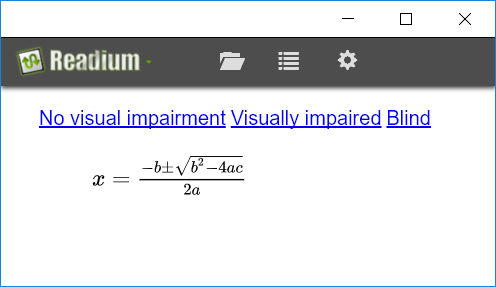
\includegraphics{EquationNormal.png}}
%\end{figure}

%\begin{figure}
%	\centerline{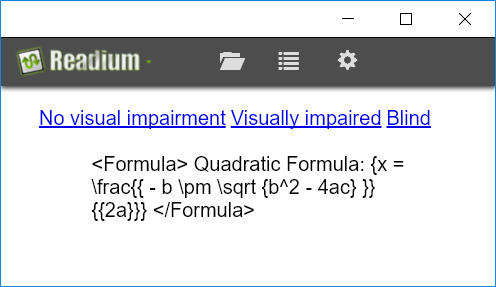
\includegraphics{EquationLatex.png}}
%\end{figure}
\vspace{-0.6cm} 
\begin{figure}
	\centering
	\begin{minipage}{0.33\textwidth}
		\centering
			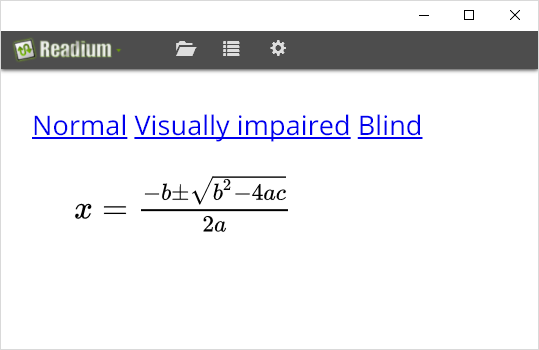
\includegraphics[width=50mm]{EquationNo.PNG} 
		\caption{EPUB in 'Normal' mode, }
		\label{fig:epub_normal}
	\end{minipage}\hfill
	\begin{minipage}{0.33\textwidth}
		\centering
		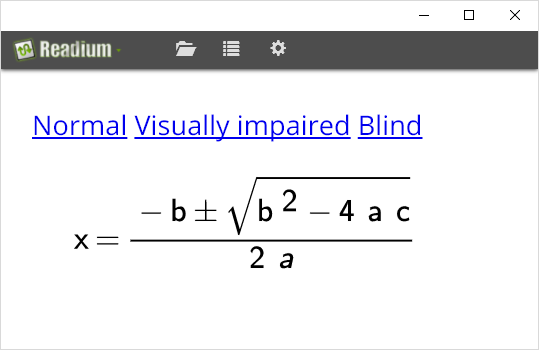
\includegraphics[width=50mm]{EquationVi.PNG} 
		\caption{in 'Visual impairment' mode,}
		\label{fig:epub_viimp}
	\end{minipage}\hfill
	\begin{minipage}{0.33\textwidth}
	\centering
			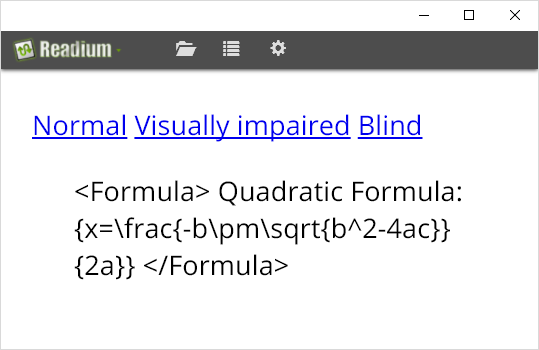
\includegraphics[width=50mm]{EquationBl.PNG} 
		\caption{and in 'Blind' mode.}
		\label{fig:epub_blind}
	\end{minipage}
\end{figure}
\vspace{-0.6cm} 
\subsection{Editor: "Accessible EPUB"}
"Accessible EPUB" is a WYSIWYG program written in C\# (. NET) that serves to create accessible EPUB documents using the switching mechanism (see figure \ref{fig:editor}). The process of creating documents should be as simple as possible so that even people with little experience in using special software can use the program. Primary target groups are, for example, teachers or implementation centres that have a need for accessible documents for different user groups.\\
When this abstract was submitted, we were just finishing the first version of our editor, which will be distributed to the first user groups during February for the first evaluation.
Some of the main features of our "Accessible EPUB" editor are:
\begin{itemize}
	\item Create an EPUB document with the switching mechanism without having to customize the source code.
	\item An equation editor which accepts LaTeX as input and inserts the MathML equivalent, SVG image and the alternative text of the equation.
	\item Ability to insert images with title, caption and alternative text.
	\item Ability to insert tables.
	\item Mark up sections using the HTML styles (h1, h2, p, etc.).
\end{itemize}
\vspace{-0.6cm} 
\begin{figure}
	\centering
	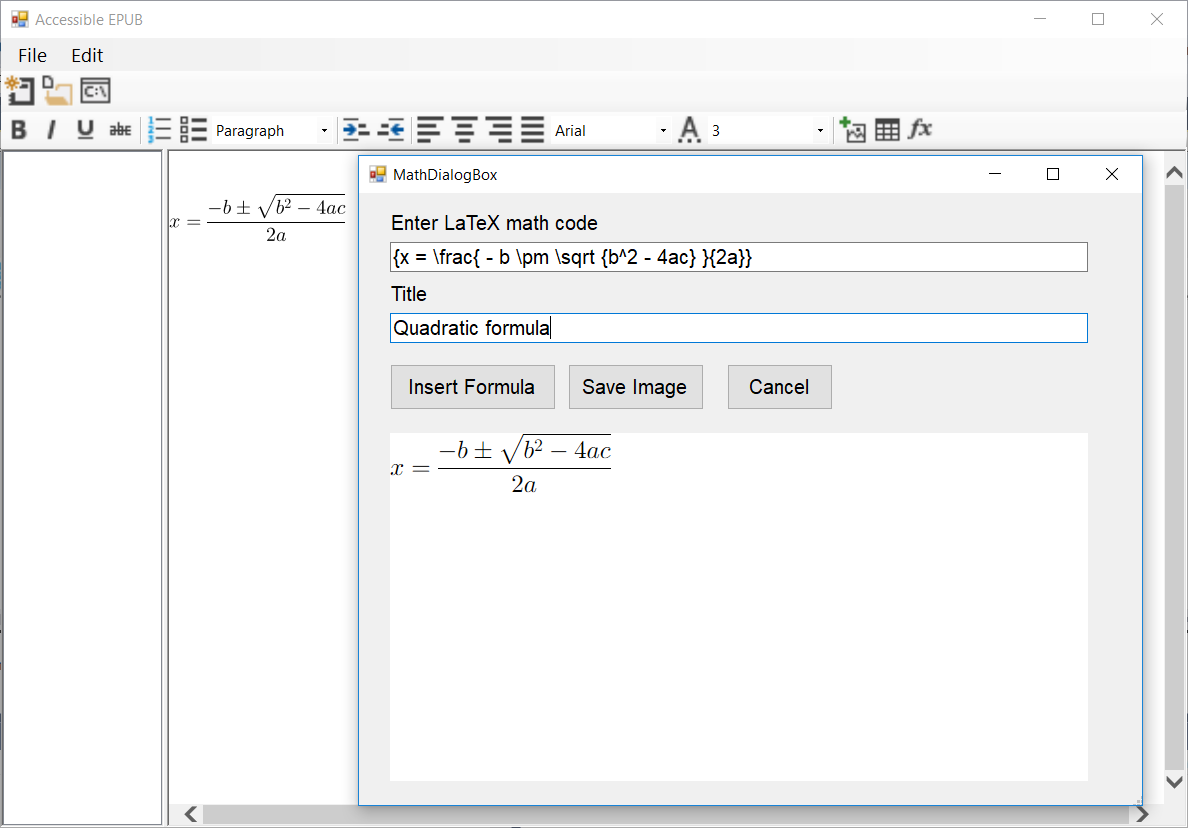
\includegraphics[height=90mm]{AccessibleEPUBequation.PNG}
	\caption{Accessible EPUB equation editor}
    \label{fig:editor}
\end{figure}
%\vspace{-1cm} 

\section{Outlook}
The final release of our "Accessible EPUB" editor and the required EPUB basedocument standard used is expected to be completed by the end of March. The camera-ready version of this paper represents the project in its entirety. This will be an insight into the structure of our EPUB format, further details about the editor and the results of an evaluation with tutors and teachers. 

%
% ---- Bibliography ----
%
\begin{thebibliography}{}
%
\bibitem[1]{webaim} WebAIM (Web Accessibility in Mind): World Laws: Introduction to Laws Throughout the World, https://webaim.org/articles/laws/world/, visited on 30.01.2018
\bibitem[2]{EPUBzone} IDPF: Understanding EPUB 3, http://epubzone.org/epub-3-overview/understanding-epub-3, visited on 29.01.2018
\bibitem[3]{EPUBspecs} IDPF: EPUB 3 Specification, http://www.idpf.org/epub/301/spec/epub-overview.html, visited on 29.01.2018
\bibitem[4]{WCAG} W3C: Web Content Accessibility Guidelines (WCAG) 2.0, https://www.w3.org/TR/WCAG20/, visited on 29.01.2018
\bibitem[5]{EPUB3bp} Garrish, M.; Gylling, M.: EPUB 3 Best Practices, 2013, O'Reilly, ISBN 1449329144, 9781449329143
\bibitem[6]{EPUB30changes} IDPF: EPUB 3 Changes from EPUB 2.0.1, http://www.idpf.org/epub/30/spec/epub30-changes.html, visited on 29.01.2018
\bibitem[7]{unified} Takaira, T.; Tani, Y.; Fujiyoshi, A.: Development of a Unified Production System for Various Types of Accessible Textbooks, Computers Helping People with Special Needs, 2016, Springer International Publishing, 381-388, ISBN 978-3-319-41264-1
\bibitem[8]{book4all} Calabr{\`o}, A.; Contini, E.; Leporini, B.: Book4All: A Tool to Make an e-Book More Accessible to Students with Vision/Visual-Impairments, HCI and Usability for e-Inclusion, 2009, Springer Berlin Heidelberg, 236-248, ISBN 978-3-642-10308-7"
\bibitem[9]{daisyAccessibility} DAISY Consortium: Baseline for Accessible EPUB3, http://www.daisy.org/baseline, visited on 29.01.2018
\bibitem[10]{voiceover} Bartalesi Lenzi, V.; Leporini, B.: Investigating an Accessible and Usable ePub Book via VoiceOver: A Case Study, Human Factors in Computing and Informatics, 2013, Springer Berlin Heidelberg, 272-283, ISBN 978-3-642-39062-3"
\bibitem[11]{enrichEPUB} Bartalesi, V.; Leporini, B.: An Enriched ePub eBook for Screen Reader Users, Universal Access in Human-Computer Interaction. Access to Today's Technologies, 2015, Springer International Publishing, 375-386, ISBN 978-3-319-20678-3
\bibitem[12]{EPUBprograms} DAISY Consortium: Tools for creating EPUB 3 files, http://www.daisy.org/daisypedia/tools-creating-epub-3-files, visited on 29.01.2018
\bibitem[13]{Sigil} Marković, S.; Schember, J.; Hendricks, K.; Massay, D.: Sigil is a multi-platform EPUB ebook editor, https://sigil-ebook.com/, visited on 29.01.2018
\bibitem[14]{WhatIsEpub3} Garrish, M.: What is EPUB 3?, 2011, O'Reilly, ISBN 9781449314545

\end{thebibliography}

\end{document}